% Created by tikzDevice version 0.12.3.1 on 2022-09-02 16:30:24
% !TEX encoding = UTF-8 Unicode
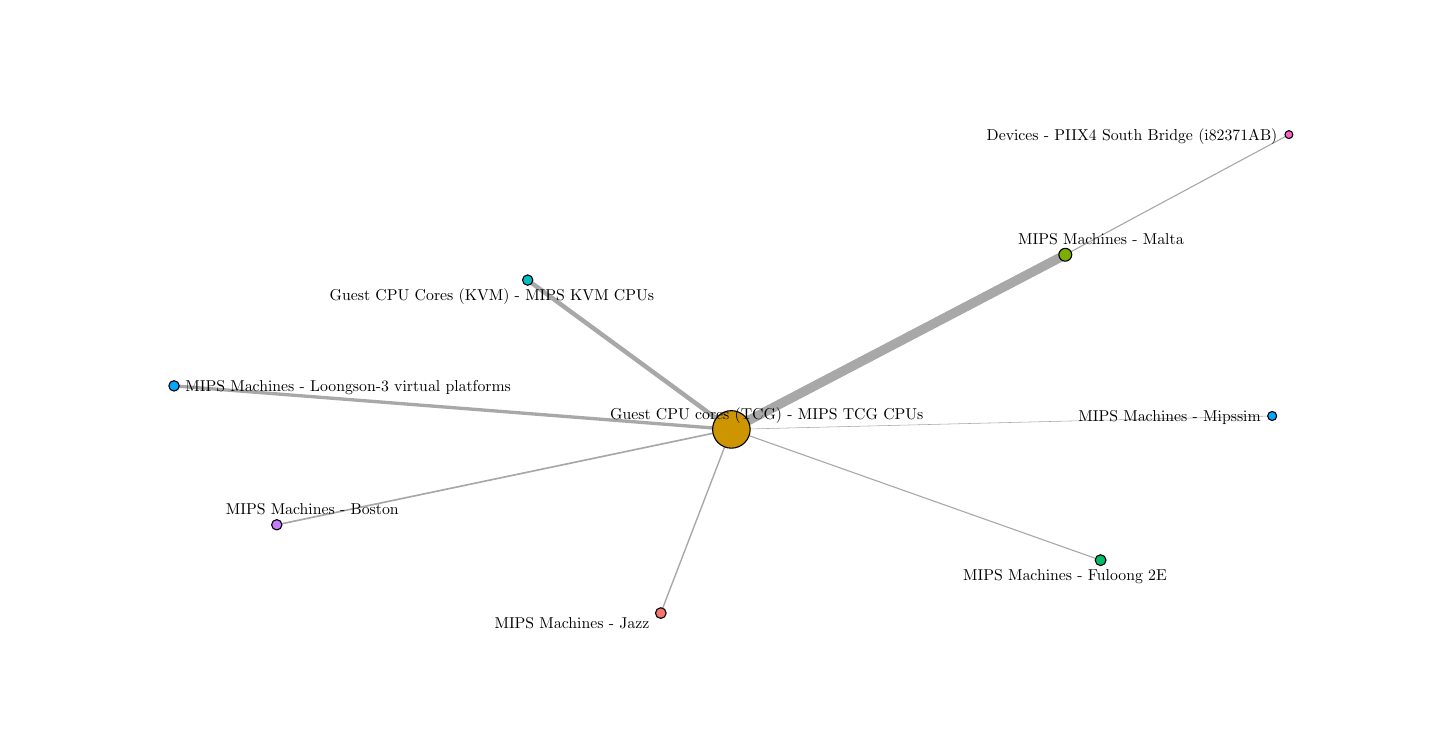
\begin{tikzpicture}[x=1pt,y=1pt]
\definecolor{fillColor}{RGB}{255,255,255}
\path[use as bounding box,fill=fillColor,fill opacity=0.00] (0,0) rectangle (505.89,252.94);
\begin{scope}
\path[clip] (  0.00,  0.00) rectangle (505.89,252.94);
\definecolor{fillColor}{RGB}{255,255,255}

\path[fill=fillColor] (  0.00,  0.00) rectangle (505.89,252.94);
\end{scope}
\begin{scope}
\path[clip] ( 32.75, 32.75) rectangle (475.89,222.94);
\definecolor{drawColor}{gray}{0.66}

\path[draw=drawColor,line width= 0.4pt,line join=round] (455.75,214.30) -- (374.94,170.88);

\path[draw=drawColor,line width= 1.6pt,line join=round] (180.68,161.73) -- (254.28,107.77);

\path[draw=drawColor,line width= 0.6pt,line join=round] (254.28,107.77) -- ( 90.01, 73.30);

\path[draw=drawColor,line width= 0.4pt,line join=round] (254.28,107.77) -- (387.70, 60.52);

\path[draw=drawColor,line width= 0.5pt,line join=round] (254.28,107.77) -- (228.78, 41.40);

\path[draw=drawColor,line width= 1.2pt,line join=round] (254.28,107.77) -- ( 52.89,123.50);

\path[draw=drawColor,line width= 3.4pt,line join=round] (254.28,107.77) -- (374.94,170.88);

\path[draw=drawColor,line width= 0.2pt,line join=round] (254.28,107.77) -- (449.70,112.62);
\definecolor{drawColor}{RGB}{0,0,0}
\definecolor{fillColor}{RGB}{255,97,204}

\path[draw=drawColor,line width= 0.4pt,line join=round,line cap=round,fill=fillColor] (455.75,214.30) circle (  1.43);
\definecolor{fillColor}{RGB}{0,191,196}

\path[draw=drawColor,line width= 0.4pt,line join=round,line cap=round,fill=fillColor] (180.68,161.73) circle (  1.87);
\definecolor{fillColor}{RGB}{205,150,0}

\path[draw=drawColor,line width= 0.4pt,line join=round,line cap=round,fill=fillColor] (254.28,107.77) circle (  6.78);
\definecolor{fillColor}{RGB}{199,124,255}

\path[draw=drawColor,line width= 0.4pt,line join=round,line cap=round,fill=fillColor] ( 90.01, 73.30) circle (  1.87);
\definecolor{fillColor}{RGB}{0,190,103}

\path[draw=drawColor,line width= 0.4pt,line join=round,line cap=round,fill=fillColor] (387.70, 60.52) circle (  1.96);
\definecolor{fillColor}{RGB}{248,118,109}

\path[draw=drawColor,line width= 0.4pt,line join=round,line cap=round,fill=fillColor] (228.78, 41.40) circle (  1.93);
\definecolor{fillColor}{RGB}{0,169,255}

\path[draw=drawColor,line width= 0.4pt,line join=round,line cap=round,fill=fillColor] ( 52.89,123.50) circle (  1.88);
\definecolor{fillColor}{RGB}{124,174,0}

\path[draw=drawColor,line width= 0.4pt,line join=round,line cap=round,fill=fillColor] (374.94,170.88) circle (  2.33);
\definecolor{fillColor}{RGB}{0,169,255}

\path[draw=drawColor,line width= 0.4pt,line join=round,line cap=round,fill=fillColor] (449.70,112.62) circle (  1.63);

\node[text=drawColor,anchor=base,inner sep=0pt, outer sep=0pt, scale=  0.57] at (399.06,212.34) {Devices - PIIX4 South Bridge (i82371AB)};

\node[text=drawColor,anchor=base,inner sep=0pt, outer sep=0pt, scale=  0.57] at (167.77,154.22) {Guest CPU Cores (KVM) - MIPS KVM CPUs};

\node[text=drawColor,anchor=base,inner sep=0pt, outer sep=0pt, scale=  0.57] at (267.08,111.32) {Guest CPU cores (TCG) - MIPS TCG CPUs};

\node[text=drawColor,anchor=base,inner sep=0pt, outer sep=0pt, scale=  0.57] at (102.84, 76.87) {MIPS Machines - Boston};

\node[text=drawColor,anchor=base,inner sep=0pt, outer sep=0pt, scale=  0.57] at (374.85, 53.05) {MIPS Machines - Fuloong 2E};

\node[text=drawColor,anchor=base,inner sep=0pt, outer sep=0pt, scale=  0.57] at (196.67, 35.77) {MIPS Machines - Jazz};

\node[text=drawColor,anchor=base,inner sep=0pt, outer sep=0pt, scale=  0.57] at (115.83,121.54) {MIPS Machines - Loongson-3 virtual platforms};

\node[text=drawColor,anchor=base,inner sep=0pt, outer sep=0pt, scale=  0.57] at (387.81,174.43) {MIPS Machines - Malta};

\node[text=drawColor,anchor=base,inner sep=0pt, outer sep=0pt, scale=  0.57] at (412.64,110.48) {MIPS Machines - Mipssim};
\end{scope}
\end{tikzpicture}
